\documentclass{beamer}
\usepackage[utf8]{inputenc}

\usepackage{utopia} %font utopia imported

\usetheme{Madrid}
\usecolortheme{default}

%------------------------------------------------------------

\title[Speech Command Project] %optional
{Speech Command Project}



\author[P Jayanth] % (optional)
{P Jayanth}

\institute[ma18btech11004] % (optional)
{MA18BTECH11004}


\date[EE5600] % (optional)
{EE5600- Speech Command Model}


%------------------------------------------------------------



%------------------------------------------------------------


\AtBeginSection[]
{
  \begin{frame}
    \frametitle{Table of Contents}
    \tableofcontents[currentsection]
  \end{frame}
}
%------------------------------------------------------------


\begin{document}

\frame{\titlepage}


%---------------------------------------------------------

\begin{frame}
\frametitle{Table of Contents}
\tableofcontents
\end{frame}
%---------------------------------------------------------


\section{Generating Data}

%---------------------------------------------------------

\begin{frame}
\frametitle{Generating Data and Storing Data}

In this Part we generate data.I used audacity to generate many samples and preprocess the data so that I get each audio sample length to 2 seconds.\\

\begin{itemize}
    \item<1-> To do so, We set Sampling Rate to 16kHz. 
    \item<2-> Generated  80 Samples of each command and saved them in respective folder.
    \item<3-> I used soundfile package to read .wav files. 
    \item<4-> Now, we Store sound-data in data\_x array and corresponding  command in data\_y array.
\end{itemize}
\end{frame}

%---------------------------------------------------------



\section{Splitting the data}

%---------------------------------------------------------
%Highlighting text
\begin{frame}
\frametitle{Splitting the data}

We need to divide data into train and test samples.So that we train the model with
train data and test the accuracy with test data so that we can check performance of our model.\\

\begin{itemize}
    \item<1-> We divided 20\% of our input data(data\_x,data\_y) as test data and remaining data into train data 
    \item<2-> We Split input data into train,test data such that both train data and test data have nearly equal proportion of each commands. 
    \item<3-> To do so,we did Stratified Sampling.
    \item<4-> Stratified Sampling is performed instead of random Sampling because Stratified Sample can provide greater precision (or less biased data that is to get equal proportions of each command) than random sample of same size.
\end{itemize}


\end{frame}
%---------------------------------------------------------

\section{Augmenting Data}
%---------------------------------------------------------
\begin{frame}
\frametitle{Augmenting Data}

Data augmentation is the process by which we create new synthetic training samples by adding small perturbations on our initial training set.\\

\begin{itemize}
    \item<1-> The objective of augmentation is to is to make our model invariant to those perturbations and enhance its ability to generalize.
    \item<2-> In order to this to work adding the perturbations must conserve the same label as the original training sample.
    \item<3-> In our case we did time-shifting, I Augment each audio sample by time shifting in 50,000 length vector filled with zeros.
    \item<4-> I took steps of 1000 to create 18 files per sample.
\end{itemize}
\end{frame}
%---------------------------------------------------------

\section{Extracting Features}
%--------------------------------------------------------
\begin{frame}
\frametitle{Extracting Features}

Extraction of features is a very important part in analyzing and finding relations between different things.\\

\begin{itemize}
    \item<1-> Sound data can be characterized with its frequencies.
    \item<2-> Mel-frequency cepstral coefficients are most prominent features in feature extractions. 
    \item<3-> We will divide our data into segments of 1024 length and then we perform various operations and we end up with 39 mel-coefficients.
    \item<4-> So our data is ready for modelling!
\end{itemize}
\end{frame}

%-------------------------------------------------------------

\section{Model}
%-------------------------------------------------------------
\begin{frame}
\frametitle{Model}

.

\begin{itemize}
    \item<1-> First we used Convolutional layers.
    \item<2-> After each CNN we added batch Normalization layers as Batch Normalization normalizes layer inputs on a per-feature basis and we know that neural networks train fast if the distribution of the input data remains similar over time.
    \item<3-> Using Bi-directional LSTM's is optimal as we have complete data.
    \item<4-> Final Output of LSTM is used to calculate importance of units of LSTM's using a Fully connected layer.
    \item<5-> Then we got Attention score at each step by doing dot-product between unit-importance and output sequences from LSTM further by doing dot-product with LSTM output sequences we get attention vectors.
    \item<6-> Then applied fully connected layer with Softmax Activation, (Since we need to classify our data into 5 classes(multinomial)) Since we need to find the command.
\end{itemize}
\end{frame}



%--------------------------------------------------------------

\section{Training}
%--------------------------------------------------------
\begin{frame}
\frametitle{Training}



\begin{itemize}
    \item<1-> We fit our data to the model we prepared before.
    \item<2-> We used Back Propagation algorithm in training our model. 
    \item<3-> The Back Propagation Algorithm updates the present layers coefficients depending on errors in next layer .
    \item<4-> Here we used Adam Optimizer to update the coefficients.
    \item<5-> Adam Optimizer is combination of RMSprop and Stochastic gradient descent with momentum.It Uses both advantages of both methods.
    \item<6-> At the end of Training we will end up with Optimal Coefficients/solution.
    
\end{itemize}
\end{frame}


%---------------------------------------------------------

%----------------------------------------------------------
\section{Testing}

%---------------------------------------------------------

\begin{frame}
\frametitle{Testing}


Inorder to know the performance of our model, we Need to test our model.

\begin{itemize}
    \item<1-> we need to prepare test data similar to train data.(else we can keep a pipeline to do this task easily)
    \item<2-> Here we sent test data as validation data in model fitting.we can see model's performance after each epoch.
    \item<3-> we can observe that it is decreasing.
\end{itemize}
\end{frame}

%-------------------------------------------------
\section{Check attention}

%---------------------------------------------------------

\begin{frame}
\frametitle{Check attention}

Here we build a sub-model from a trained model but we add Attention Soft-max layer
as additional output layer.\\
\begin{itemize}
    \item<1-> Now we pass our test data to our new model to the predict method.
    \item<2-> Then we plotted log of Attention Scores and corresponding input vector before taking MFCC on other axes.
    \item<3-> We can see that attention are high at high informative parts.
\end{itemize}

\end{frame}
%----------------------------------------------------
\begin{frame}
\frametitle{Check attention}
\begin{figure}[h]
    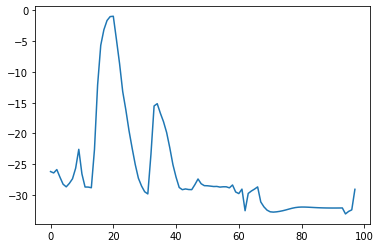
\includegraphics[width=\columnwidth]{log.png}
    \caption{plot of log attention scores and corresponding input vectors before taking MFCC's on different axes}
\end{figure}\\


    
\end{frame}
%--------------------------------------------------------------
\begin{frame}
\frametitle{Check attention}
\begin{figure}[h]
    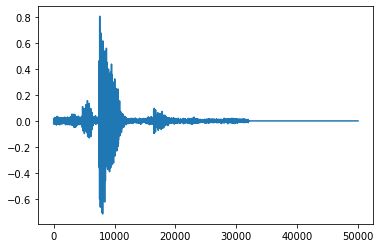
\includegraphics[width=\columnwidth]{raw.png}
    \caption{Raw Sample}
\end{figure}\\
\end{frame}
%----------------------------------------------------------------

\begin{frame}
\frametitle{END}
\begin{align*}
    The-END 
\end{align*}
    
\end{frame}

%---------------------------------------------------------


\end{document}